\chapter{Test}

Projektet stiller krav om løbende udvikling og ikke mindst krav om kvalitet. 
Automatiserede tests har dermed været et naturligt valg. De automatiserede test har konstant og systematisk hjulpet os som udviklere til at sørge for, at kvaliteten i vores system opretholdes, når ny funktionalitet er blevet tilføjet. Der er specielt blevet lagt fokus på unit test i system. Detektion af fejl i tidligere kode, når ny kode tillægges er ligeledes en afgørende faktor for dette valg.

\section{Continuous Integration}
Projektet er sat op, så der benyttes continuous integration, så projektet bliver bygget på en ekstern server, hver gang der bliver tilføjet en ændring til projektet via git. CI er blevet brugt for at undgå integrations problemer, der kan opstå, når flere gruppemedlemmer arbejder samtidig på samme projekt.
I forbindelse med at projektet bliver bygget på CI-serveren bliver de projektets test samtidig kørt.

TeamCity blev anvendt som CI-server, hvor der blev opsat et  projekt, der blev sat til at pege på gruppens github-repository. Projektet blev sat op til, at hver gang der blev "pushed" til reopistoriet skulle TeamCity kører to "Build Steps". I første step blev projektet bygget ved brug af MSBuild Tools 2015. Hvis det første skridt gik godt blev anden step udført, der bestod i at køre Test-projektets NUnit-tests. Testene blev kørt ved brug af en NUnit.ConsoleRunner, der var blevet installeret som en NuGet-Package i projektet.  
CI-projeket blev også tilknyttet en dotCover-test, der skulle fungere som et pejlemærke for, hvor stor en del af projektet testene dækker. Da der ikke var nogen specielle krav til Coverage-analysen blev JetBrains standard dotCover fil benyttet.

\noindent Nedenunder på figur \ref{fig:TeamCityTest} kan et eksempel af et build på TeamCity serveren ses. 
\begin{figure}[ht!]
	\centering
	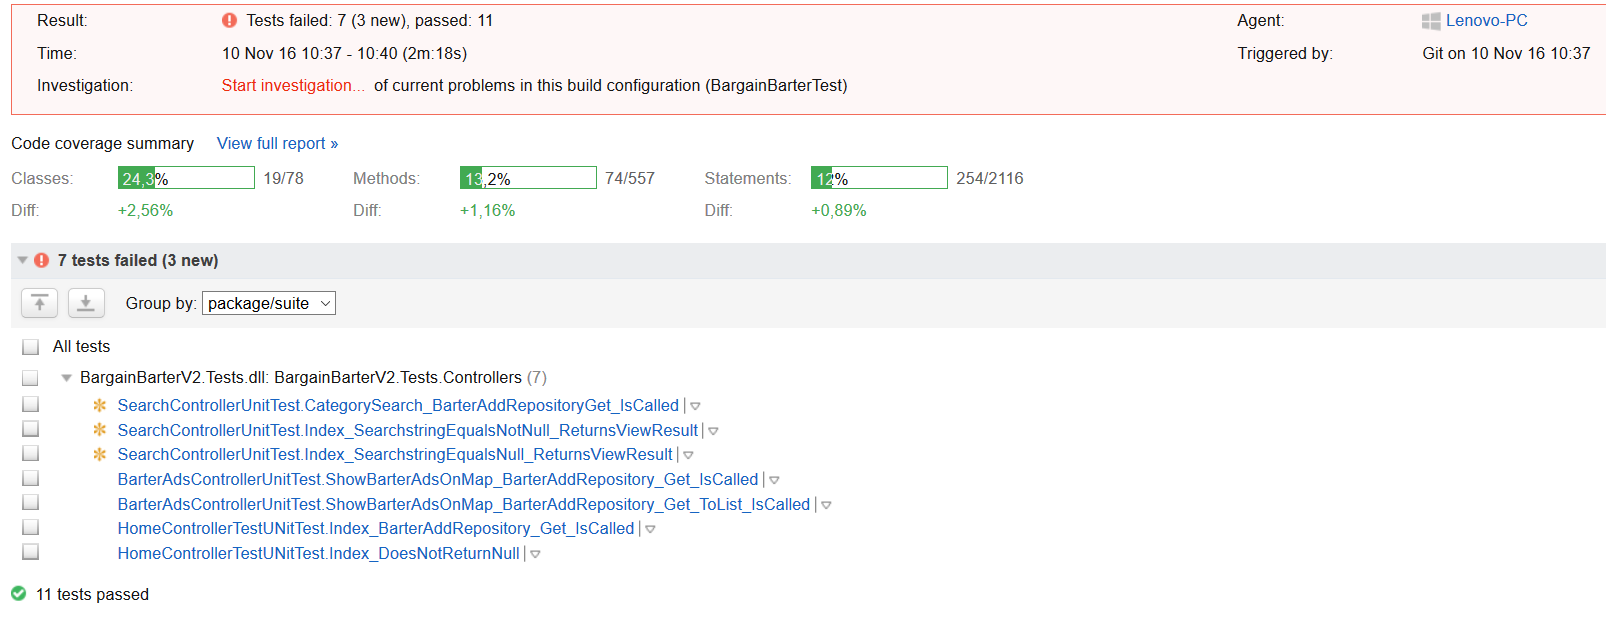
\includegraphics[width=120mm]{figures/TeamCityTest.png}
	\caption{Testresultat på baggrund af kørte test på TeamCity}
	\label{fig:TeamCityTest}
\end{figure}



\section{Unit Tests af controllerne}
Da systemet i starten af udviklingsfasen kun indeholdt meget minimal buisness-logic, ligger størstedelen af funktionaliteten i controllerne i MVC strukturen. 
Denne struktur med at lægge funktionalitet i controller blev fastholdt igennem udviklingsfasen. Dette blev erfaret som en dårlig beslutning, da controllerne ofte udover buisness-logikken også benyttede sig af web-specifikke metoder \footnote{HttpContext-metoder}, der gør unit test på disse metoder tæt på umulig. Designet skulle derfor have været refaktoreret, således at mere af buisness-logikken var blevet flyttet til et separat buisness-lag, så denne del af systemet kunne være blevet testet.
De controllere, som kunne testes, er således også den vigtigste at teste. Databasen i sig selv er svær at teste, og views i MVC'en kan nærmest ikke testes. Det der reelt kan testes er derfor, hvad controllerne giver videre til deres views, og således ikke selve views'ne.\\ I Controllerne er der flere ting der er væsentligt at teste.
\begin{itemize}
	\item Hvad gives med i viewbagen
	\item Buisness-logic funktioner som controllerne bruger
	\item At de korrekte fejl bliver kaldt når controllerne giver ugyldige værdier
	\item De enkelte redirects bliver kaldt korrekt
	\item At de enkelte controllers returnerer views
\end{itemize}       
Disse er de udvalgte ting som er vurderet til at give mening at teste på.

Den fulde liste af test kan ses nedenfor.
\setlength{\arrayrulewidth}{0.3mm}
\setlength{\tabcolsep}{2pt}
\renewcommand{\arraystretch}{1.5}
\begin{table}[H]
	\begin{tabular}{ | p{3.0cm} | p{5.5cm} | p{8.0cm} | }
		\hline
		\textbf{Controller} & \textbf{Test} & \textbf{Beskrivelse} \\
		\hline
		BarterAds-Controller &  Index\_RedirectsToController-\_HomeActionIndex & Tester om controlleren faktisk kalder der rigtige view til Home. \\
		
		& ShowBarterAdsOnMap-\_BarterAddRepository-\_Get\_IsCalled & Tester om controller kalder den rigtige metode for at vise alle barteradds på kortet\\
	
		& Details\_NullId\_Returns-\_BadRequest & Tester om hvis metoden Details får Null, som id, så returnerer controlleren en BadRequest, kode 400. \\
		&Create\_DoesNot\_Return\_Null& Tester, at create controller retunerer et view \\
		& Edit\_NullId\_Returns\_BadRequest &  Tester om hvis metoden Edit får Null, som parameter, så returnerer controlleren en BadRequest, kode 400. \\
		& Delete\_NullId\_Returns\_BadRequest & Tester om hvis metoden Delete får Null, som parameter, så returnerer controlleren en BadRequest, kode 400. \\
		\hline
		ManageController & ChangePassword\_DoesNotReturnNull &Tester, at ChangePassword metoden retuner et view, der er forskellig fra null\
		\\
		\hline
		HomeController & Index\_BarterAddRepository-\_Get\_IsCalled & Tester om den metode der viser alle barteradds på Index siden, bliver vist. \\
		& Index\_DoesNotReturnNull & Tester, at index metoden  retuner et view, der er forskellig fra null\\
		& AboutDoesNotReturnNull & Tester, at About-metoden  retuner et view, der er forskellig fra null \\
		& ContactDoesNotReturnNull &  Tester, at Contact-metoden retuner et view, der er forskellig fra null  \\
		\hline
		SearchController & Search\_Calls-\_BarterAdsRepository & Tester om den BarterAddRepository bliver kaldt når man søger efter en bestemt ting \\
		& CategorySearch\_Calls-\_BarterAdsRepository & Tester om BarterAdsRepository anvendes at og bliver kaldt når man vælger kategori \\
		& Index\_DoesNotReturnNull & Tester, at Index-metoden retuner et view, der er forskellig fra null\\
		& Index\_SearchstringIsNull\_ReturnsNotNull & Tester om, at Index-metoden retunerer et view, der giver mening på trods af  den modtager null som paramter\\
		& Categorysearch\_SearchstringIsNonEmpty\_ResultIsNotNull & Tester om, at Categorysearch-metoden retunerer et view, der giver mening, når det modtager en paramter\\
		\hline
		HelperFunctions & CalculateAverage\_Test & Tester om CalculateAverage udregner gennemsnittet rigtigt på baggrund af en nogen kontrol-værdier. \\ &  CalculateUserAvg\_Test & Tester om CalculateuserAvgRating kan udregne udregne gennemsnittet rigtig for en bruger på baggrund af en liste af FinishedTrades\\
		\hline
		HelperFunctions Distance & GetDistance\_Test & Tester om en adresse kan konverteres til koordinater og om distancen mellem koordinaterne er rigtig.\\
		\hline
	\end{tabular}
\end{table}

Det er væsentligt at pointere hvordan disse test bliver lavet isoleret, således at controllerne ikke er afhængige af DAL-laget.

\subsection{Unit test igennem DAL}

Som nævnt spiller design og test i høj grad sammen. Dette er også grunden til, at der i projektet er blevet anvendt repository pattern, der uddybes i afsnit \ref{ch:Design}. På figur \ref{fig:UnitOfWorkMock} kan det ses, hvordan repository-pattern og UnitOfWork i høj grad spiller sammen med test af systemet. Det er muligt at teste systemet direkte gennem dbcontexten som ses uden Repository pattern. Men dette er ikke en selvfølgelighed, og ved ændring af database teknologi vil alle tests skulle skrives om. Dette er ikke ønsket, da selve unit testene skal teste om en klasse kalder korrekt ned i andre klasser. En unit test skal også være genbrugelig, så en god unit test burde ikke skulle skrives om på baggrund af systemændringer. Unit testene skal ikke teste om kaldene ned i de andre klasser rent faktisk virker. Det er ikke controllerne i MVC-mønsteret, der har ansvar for, at database kaldene virker. Derfor bruges UnitOfWork i testene som en mock på baggrund af, at der benyttes dependency injection i systemet. Mocken af UnitOfWork er den, som controlleren kalder ned i. På den måde ved brug af repository pattern opnås, at controllerne kan testes uafhængigt af Data Access Laget og selve databasen.

\begin{figure}[H]
	\centering
	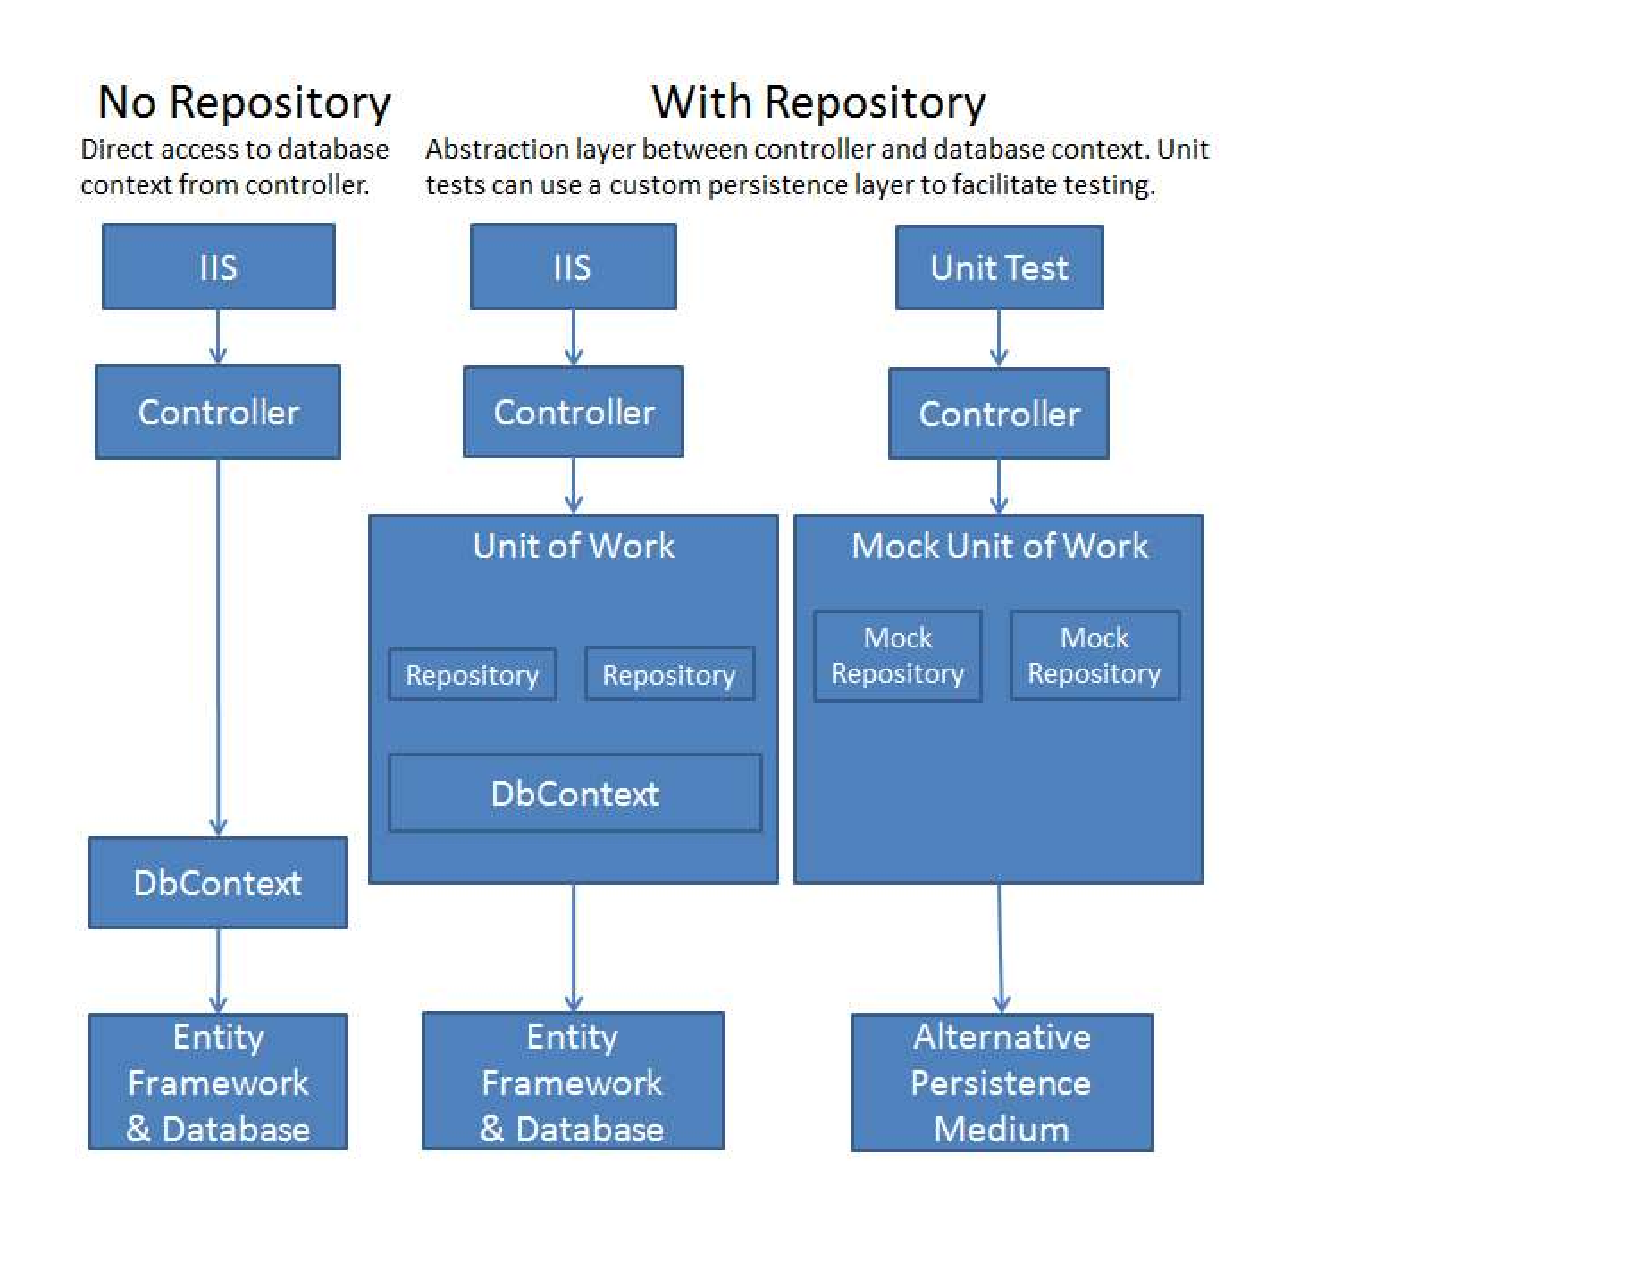
\includegraphics
	[width=165mm]{figures/RepsitoryTestFigure.PDF}
	\caption{Unit test med UnitOfWork-Mock \cite{UOFTest}}
	\label{fig:UnitOfWorkMock}
\end{figure}

\section{Integrationstest}
%Efterfulgt af at de enkelte unit tests af controllersne, testes integrationen af controllerne med den relle database. Da samhørigheden af de forskellige controllers er forholdsvis lav er integrationstesten en relativ simpel opgave, hvor der kun er taget de enkelte dele der er vurderet til at give mening med.    
%
%INDSÆT DPTREE
%%\begin{figure}[H]
%%	\centering
%%	\includegraphics
%%	[width=165mm]{figures/DependencyTree.PDF}
%%	\caption{DependencyTree}
%%	\label{fig:DependencyTree}
%%\end{figure}
%
%\noindent Det sidste skridt er selvfølgelig at tests viewne, hvor der er lavet en user experience vurdering, og naturligvis en acceptest der kan ses i efterfølgende afsnit
Efterfulgt af unit test de enkelte controller, skal integrationen mellem de forskellige dele af systemet testes. Der er dog imidlertid ikke den store afhængighed mellem de forskellige controllers i systemet, hvilket MVC også lægger op til. Det ville derfor valgt ikke at lave en integrationstest af systemet, da der reelt er få dele af systemet, hvor man kan teste for afhængigheden mellem de forskellige dele af systemet. \\

\section{Manuelle tests}
Grundet applikationens GUI og arkitektur har det ikke været muligt at automatisere alle tests. Derfor har de automatiserede unit tests været suppleret meget med manuelle tests. Dette har på simpel vis foregået ved, at en tester har klikket rundt på hjemmesiden og bekræftet om den nyimplementerede funktionalitet har virket. I dette afsnit vil der følge et par eksempler på, hvordan de manuelle test har fundet sted. Ikke alle manuelle tests er beskrevet her, da det ville være for uoverskueligt. Men generelt gælder det, at stort set alt funktionalitet er blevet testet manuelt.

\subsection{Test af byttehandel}
Byttehandel funktionaliteten er blevet testet ved, at der for selve byttehandlen er blevet defineret en række af punkter, der skal gennemføres i forbindelse med en byttehandel. Disse punkter udgøre tilsammen et bytteflow. 
Bytteflowet kan ses på figur \ref{fig:bytteflow}. 
\begin{figure}[H]
	\centering
	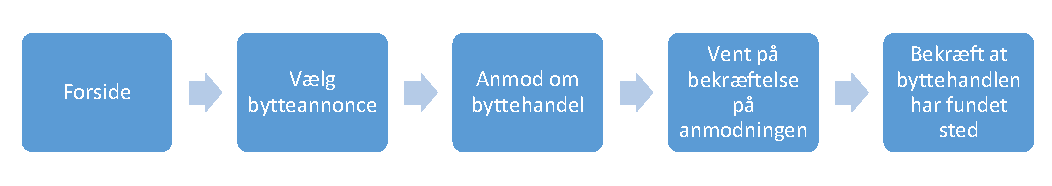
\includegraphics
	[width=140mm]{figures/bytteflow.pdf}
	\caption{Flow over en byttehandel i BargainBarter}
	\label{fig:bytteflow}
\end{figure}
Når bytteflowet skulle testes blev dette gjort på baggrund af bytteflowet. Bytteflowet blev slavisk gennemført og på baggrund af en byttehandel var gennemført eller ej, kunne byttehandel funktionaliteten be- eller afkræftes.

\subsection{Test af Chat}
Chat funktionaliteten er skrevet i javascript, hvilket har gjort, at den ikke kunne testes automatisk ved brug af NUnit. 
Chat funktionaliteten er derfor blevet testet manuelt på baggrund af nedenstående flow, der ses på figur \ref{fig:chatflow}.

\begin{figure}[H]
	\centering
	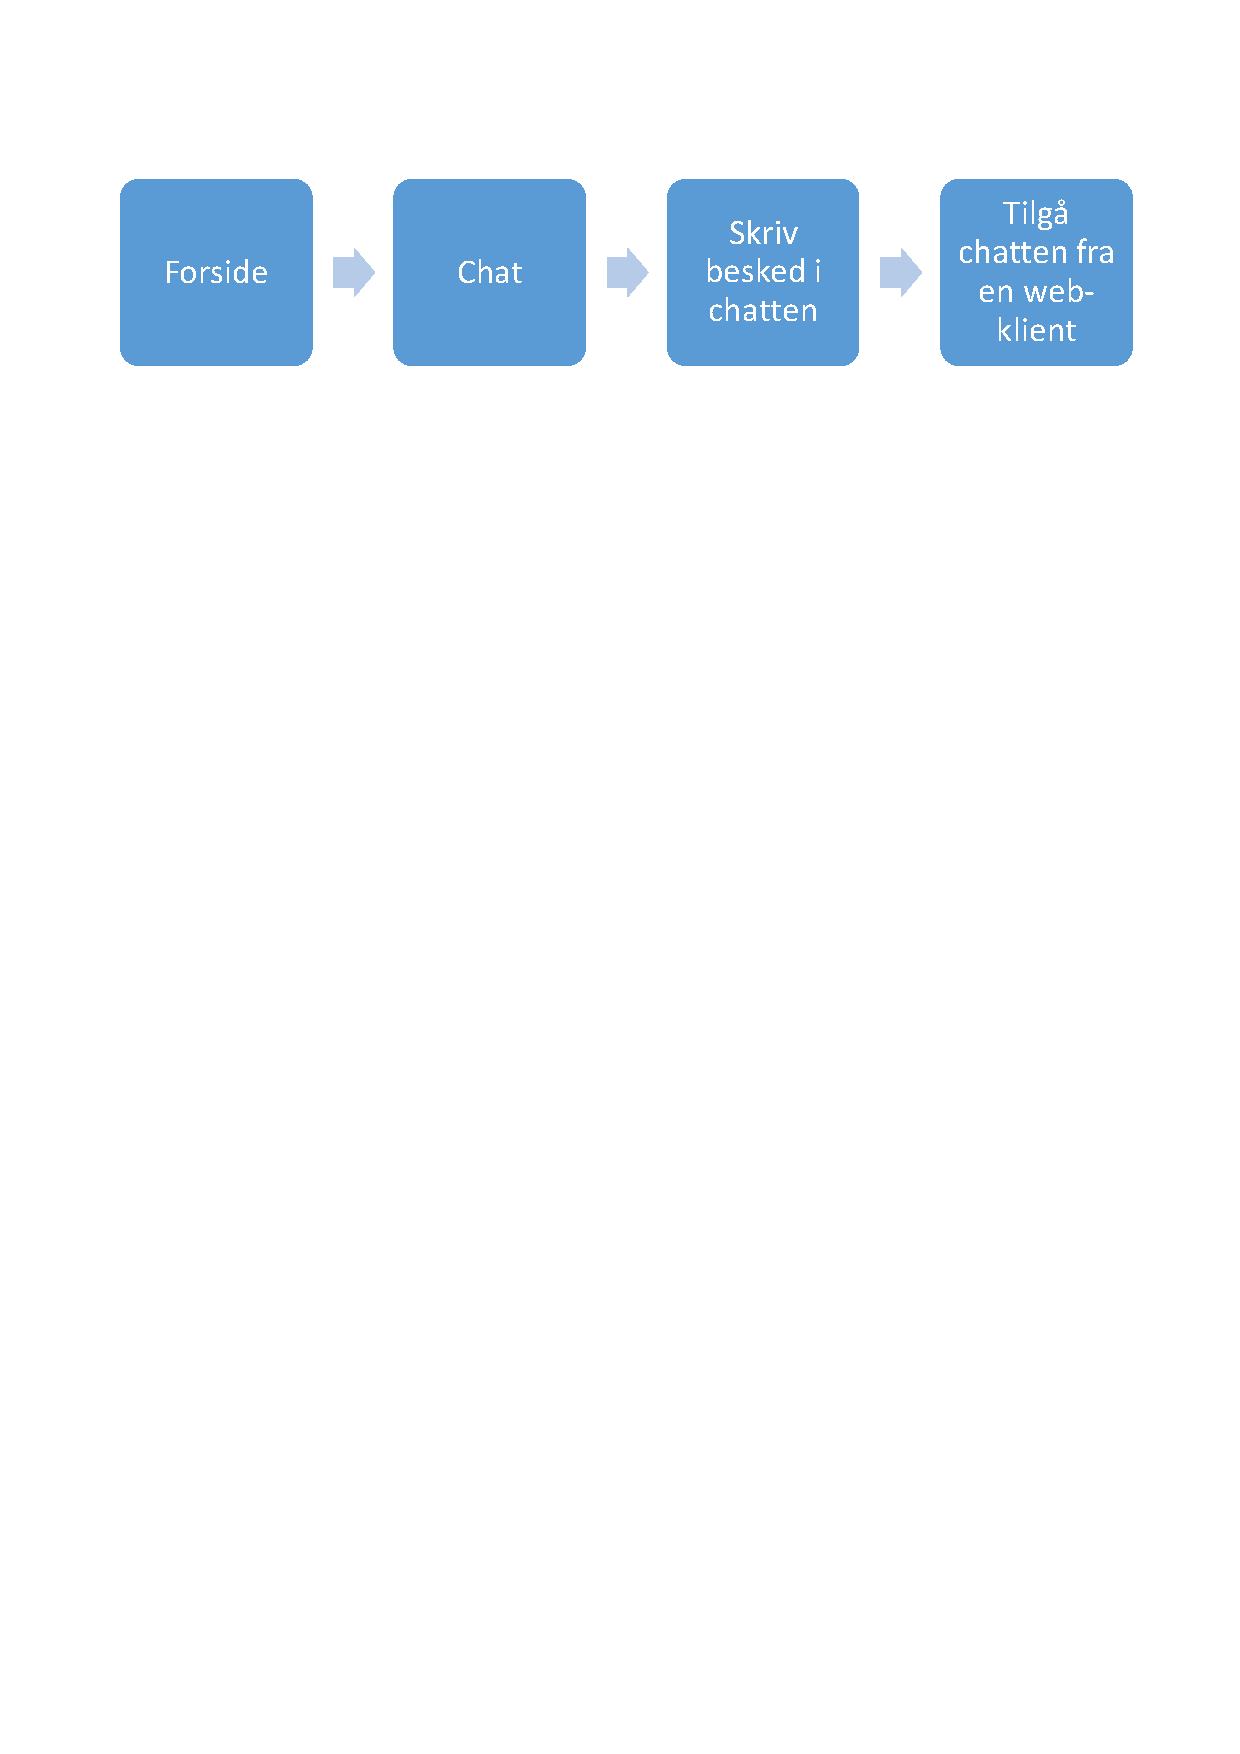
\includegraphics
	[width=140mm]{figures/chatflow.pdf}
	\caption{Flow over chatten på BargainBarter}
	\label{fig:chatflow}
\end{figure}


Chatten blev testet på baggrund af flowet fra figur \ref{fig:chatflow}.Resultatet af chat-testen set fra en anden s web-klient ses på figur \ref{fig:chattest}.
\begin{figure}[H]
	\centering
	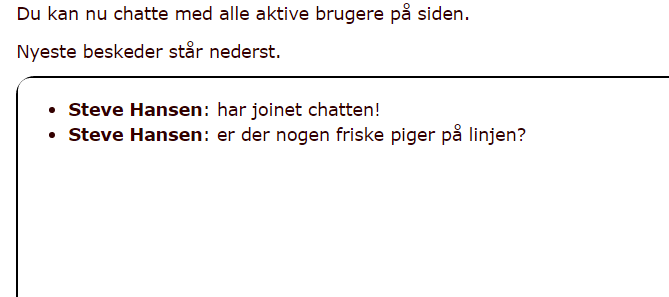
\includegraphics
	[width=140mm]{figures/ChatTest.png}
	\caption{Test af chat}
	\label{fig:chattest}
\end{figure}

\subsection{Opret annonce}
Opret annonce funktionaliteten er blevet testet manuelt på baggrund af nedenstående annonceflow, der ses på figur \ref{fig:annonceflow}.

\begin{figure}[H]
	\centering
	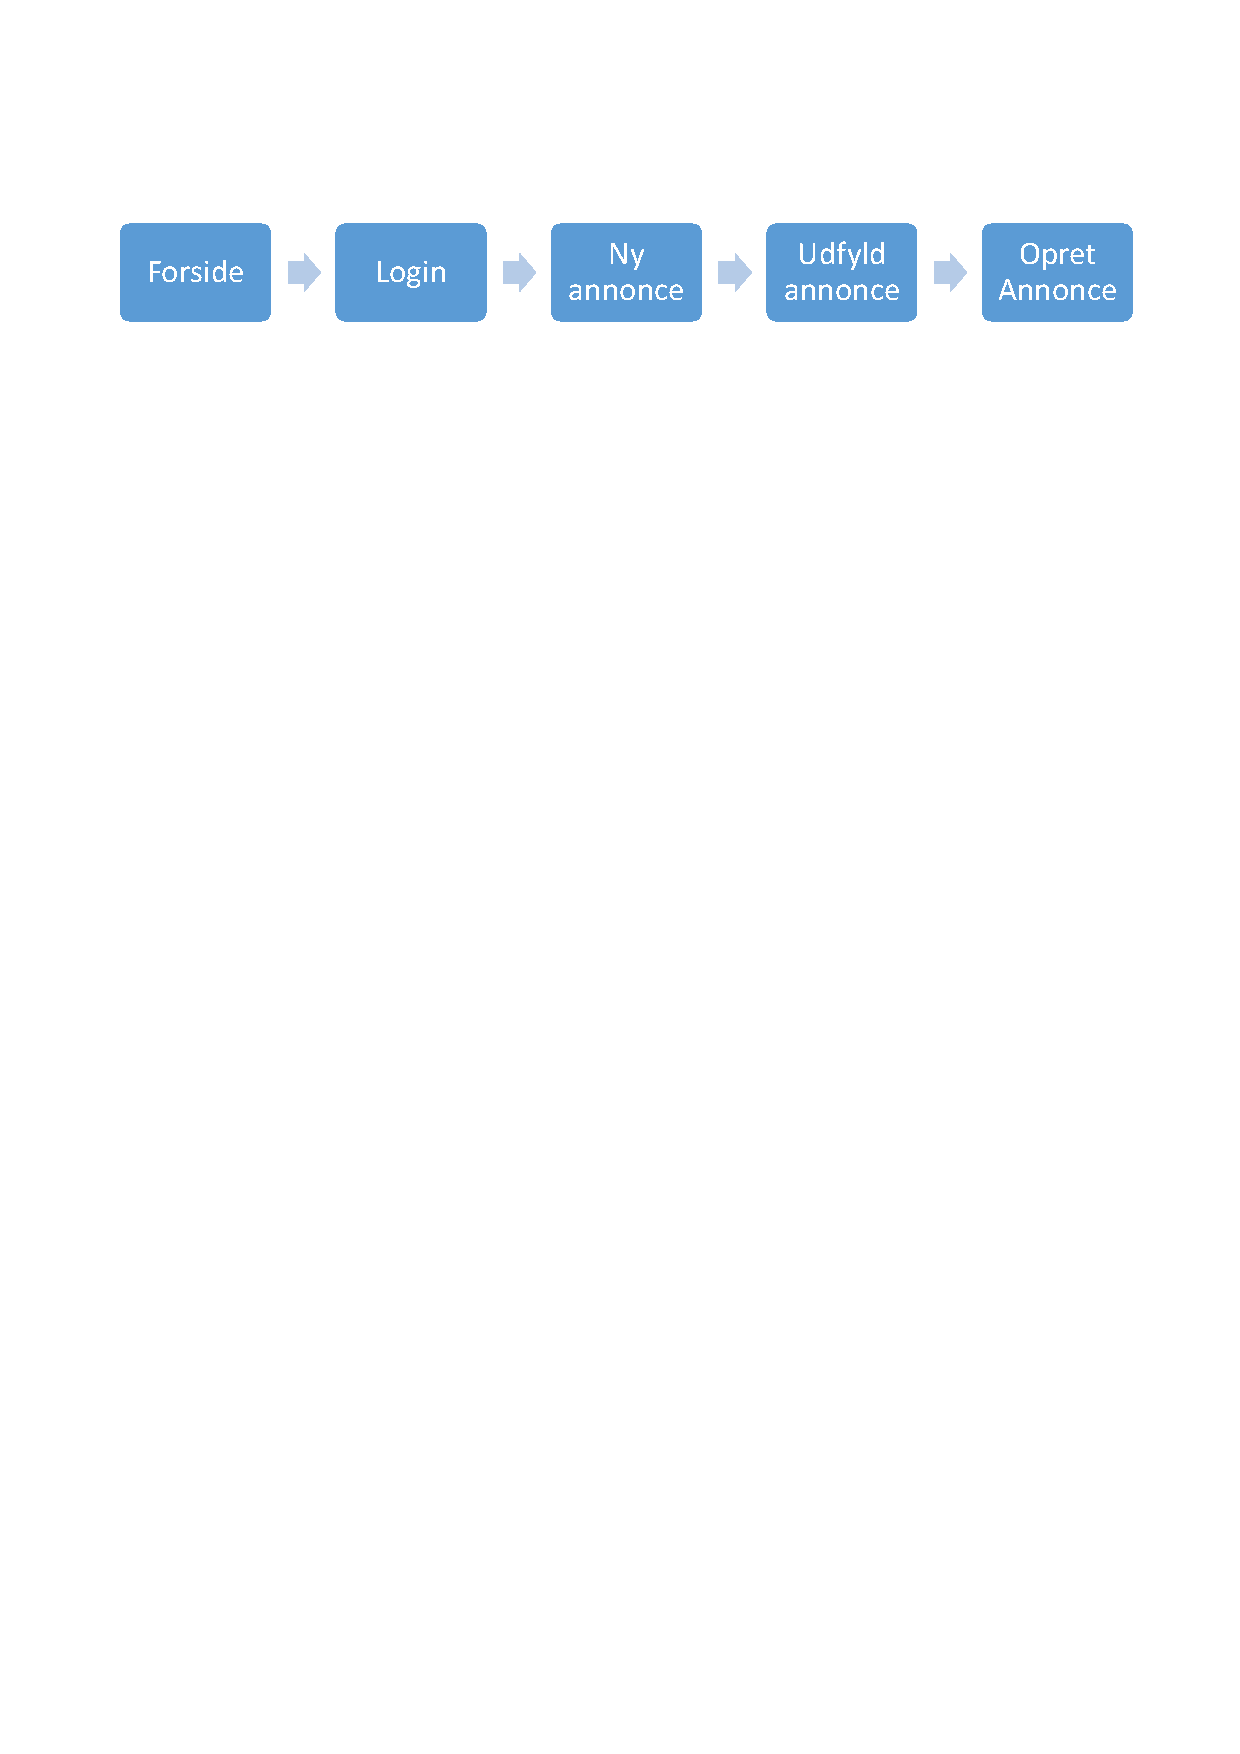
\includegraphics
	[width=140mm]{figures/annonceflow.pdf}
	\caption{Flow over oprettelse af annonce på BargainBarter}
	\label{fig:annonceflow}
\end{figure}

Overstående flow blev gennemført, hvor det til sidst blev bekræftet, at der var blevet oprettet en annonce for brugeren.